\section{A New Framework for On-Stack Replacement}

Modern language runtimes dynamically adapt the execution to the actual workload, maintaining different versions of the code generated with different, often speculative, optimizations. For this reason, they typically implement on-stack replacement mechanisms to dynamically transfer execution between them {\em while} a version of the method to optimize is still running.

Pioneered in the SELF language runtime in the early 90's, OSR mechanisms have drawn considerable attention from the community of VM builders as the Java language grew popular. OSR is nowadays used in a relevant number of virtual machines to implement optimization techniques such as profile-driven and deferred compilation, and can also be employed to support debugging of optimized code.

\noindent OSR can be a very powerful tool for implementing dynamic languages, for which most effective optimization decisions can typically be made only at run time, when critical information such as type and shape of objects becomes available. In this scenario, OSR becomes useful also to perform deoptimization, i.e. when the running code has been speculatively optimized and the assumption used for the optimization does not hold anymore, the optimized function is interrupted and the execution continues in a safe version of the code.

In this thesis, we propose a general-purpose, target-independent framework for OSR. Specific goals of our solution include:
\begin{itemize}[parsep=0pt]
\item The ability for a function reached via OSR to fire an OSR itself: this would allow switching from a base function $f$ to an optimized function $f'$, and later on to a further optimized version $f''$, and so on.
\item Supporting deoptimization, i.e., transitions from an optimized function to a less optimized function from which it was derived.
\item Supporting transitions at arbitrary program points, including those that would require adjusting the transferred program state to resume the execution in the OSR target function.
\item Supporting OSR targets either generated at run-time (e.g., using profiling information) or already known at compilation time.
\item Hiding from the front-end that generates the different function versions all the implementation details for handling OSR transitions between them.% at specific points.
\end{itemize}

\noindent We show the feasibility of our approach by implementing \osrkit, a prototype library for the MCJIT just-in-time compiler from the LLVM compiler infrastructure.

\subsection{Approach}

The key to generality and platform-independence in our approach is to express the OSR machinery entirely at intermediate representation (IR) level, without resorting to native-code manipulation or special intrinsics of a compiler.

\ifdefined\noauthorea
\begin{figure}[hb]
\begin{center}
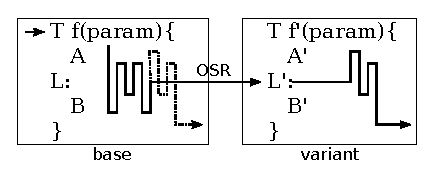
\includegraphics[width=0.7\textwidth]{figures/osr-dynamics/osr-dynamics.eps}
\caption{\protect\label{fig:osr-dynamics} On-stack replacement dynamics: control is transferred via OSR from a point \textsf{L} of a base function \textsf{f} to a point \textsf{L'} in a variant \textsf{f'} of \textsf{f}.}
\end{center}
\end{figure}
\fi

\noindent Consider the generic OSR scenario shown in \myfigure\ref{fig:osr-dynamics}. A base function \fbase\ is executed and it can either terminate normally (dashed lines), or an OSR event may transfer control to a variant \fvariant, which resumes the execution. The decision of whether an OSR should be fired at a given point \osrpoint\ of \fbase\ is based on an {\em OSR condition}. A typical example in JIT-based virtual machines is a profile counter reaching a certain hotness threshold, which indicates that \fbase\ is taking longer than expected and is worth optimizing. Another example is a guard testing whether \fbase\ has become unsafe and execution needs to fall back to a safe version \fvariant. This scenario includes deoptimization of functions generated with aggressive speculative optimizations.

Several OSR implementations adjust the stack so that execution can continue in \fvariant\ with the current frame \cite{Chambers91, Chambers92, Holzle92, Suganuma06}. This requires manipulating the program state at machine-code level and is highly ABI- and compiler-dependent. A simpler approach, which we follow in this thesis, consists in creating a new frame every time an OSR is fired, essentially regarding an OSR transition as a function call~\cite{Lameed13,Pizlo14}. Our solution targets two general scenarios:
\begin{enumerate}[parsep=0pt]
 \item {\em resolved OSR}: \fvariant\ is known before executing \fbase\ as in the deoptimization example discussed above;
 \item {\em open OSR}: \fvariant\ is generated when the OSR is fired, supporting deferred and profile-guided compilation strategies.
\end{enumerate}

\noindent In both cases, \fbase\ is instrumented before its execution to incorporate the OSR machinery. We call such OSR-instrumented version \fosrfrom.

In the resolved OSR scenario (see \myfigure\ref{fig:osr-resolved}), instrumentation consists of adding a check of the OSR condition and, if it is satisfied, a tail call that fires the OSR. The called function is an instrumented version of \fvariant, which we call \fosrto. We refer to \fosrto\ as the {\em continuation function} for an OSR transition. The assumption is that \fosrto\ produces the same side-effects and return value that one would obtain by \fbase\ if no OSR was performed. Differently from \fvariant, \fosrto\ takes as input all live variables of \fbase\ at \osrpoint, executes an optional {\em compensation code} to fix the computation state ({\tt comp\_code}), and then jumps to a point \textsf{L'} from which execution can continue.

\ifdefined\noauthorea
\begin{figure}[b]
\begin{center}
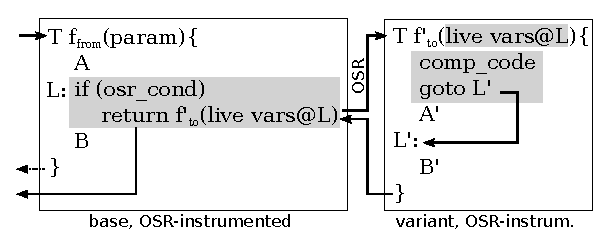
\includegraphics[width=0.7\textwidth]{figures/osr-resolved/osr-resolved.eps}
\caption{\protect\label{fig:osr-resolved} Resolved OSR scenario.}
\end{center}
\end{figure}
\fi

%Compensation code adds flexibility to our framework, as it extends the range of points where OSR transitions can be fired. In fact, the OSR practice often makes the conservative assumption that execution can always continue with the very same program state as the base function. This assumption can however be restrictive, as it may reduce the number of program locations eligible for OSR (i.e., one has to wait to a point where the states would correspond). Our solution provides a front-end with means to encode a compensation code, tailored to the specific optimizations involved between two function versions, that is needed to adjust the program state and perform an OSR at an arbitrary given location.

Compensation code adds flexibility to our framework, as it extends the range of points where OSR transitions can be fired. In fact, the OSR practice often makes the conservative assumption that execution can always continue with the very same program state as the base function. %This assumption may however reduce the number of OSR opportunities, e.g., one has to wait to a point where the states would correspond.
This assumption can however be restrictive, as it may reduce the number of program locations eligible for OSR (i.e., one has to wait to a point where the states would realign). Our solution provides a front-end with means to encode a glue code, tailored to the specific optimizations involved between two function versions, to adjust the program state and perform an OSR transition. This code can be used, for instance, to modify the heap, or to reconstruct values for variables that are live at \textsf{L'} but not at \textsf{L}.

The open OSR scenario is similar, with one main difference (see \myfigure\ref{fig:osr-open}): instead of calling \fosrto\ directly, \fosrfrom\ calls a stub function \fstub, which first creates \fosrto\ and then calls it. Function \fosrto\ is generated by a function {\tt gen} that takes the base function \fbase\ and the OSR point \osrpoint\ as input. The reason for having a stub in the open OSR scenario, rather than directly instrumenting \fbase\ with the code generation machinery, is to minimize the extra code injected into \fbase. Indeed, instrumentation may interfere with optimizations, e.g., by increasing register pressure and altering code layout and instruction cache behavior. \mynote{JIT compilation?}

\ifdefined\noauthorea
\begin{figure}[t]
\begin{center}
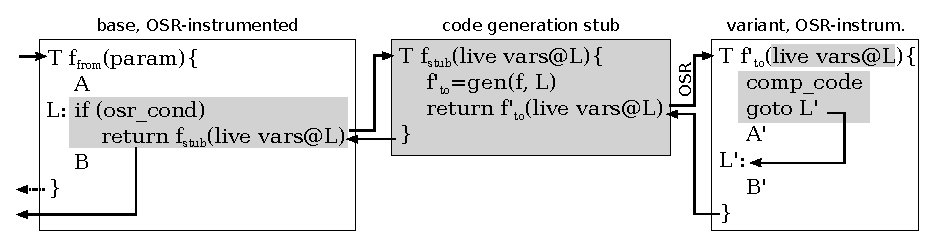
\includegraphics[width=1.0\textwidth]{figures/osr-open/osr-open.eps}
\caption{\protect\label{fig:osr-open} Open OSR scenario.





}
\end{center}
\end{figure}
\fi

\subsection{LLVM Implementation}

The LLVM compiler infrastructure~\cite{Lattner04} provides a Just-In-Time compiler called MCJIT that is currently being used for generating optimized code at run-time in virtual machines for dynamic languages. MCJIT is employed in both industrial and research projects, including Webkit's Javascript engine, the open-source Python implementation Pyston, the Rubinius project for Ruby, Julia for high-performance technical computing, McVM for MATLAB, CXXR for the R language, Terra for Lua, and the Pure functional programming language. The MCJIT compiler shares the same optimization pipeline with LLVM front-ends for static languages such as \clang, and it provides dynamic features such as native code loading and linking, as well as a customizable memory manager for code and data sections.

Currently VM builders using MCJIT are required to have a deep knowledge of the internals of LLVM in order to mimic an OSR mechanism. In particular, they can rely on two experimental intrinsics, {\em Stackmap} and {\em Patchpoint}, to inspect the details of the compiled code generated by the back-end and to patch it manually with a sequence of assembly instructions. A {\em Stackmap} is used to record the run-time location (i.e., register, stack offset or constant) for a set of variables (e.g., the set of live variables) at a given IR instruction. The intrinsic generates no code in place\footnote{Although a front-end can ask LLVM to insert a number of NOP instructions into the function to prevent overwriting program text or data outside the function during the run-time patching.}, as the back-end emits its data into a designated section in the object code. A Stackmap allows the runtime to disruptively patch the original code in response to an event triggered from outside, thus executing a new code sequence when the location for the original IR instruction is reached. A {\em Patchpoint} instead creates a function call to a target typically not known at compile time, and implies a StackMap generation to track the run-time location for the set of variables given as argument. A Patchpoint reserves space for injecting new code (e.g., to update the target of the call), so that the other instructions in the function are preserved. An example application of the Patchpoint intrinsic is the implementation~\cite{Pizlo14} of an inline caching mechanism~\cite{Deutsch84} for polymorphic method dispatch in the WebKit JavaScript engine. Both intrinsics are currently marked as experimental, and are treated along the optimization pipeline as instructions that can potentially read and write all memory\footnote{A {\tt store} instruction clearly cannot be moved across a Stackmap, but also a {\tt load} must be handled conservatively (i.e., cannot be hoisted above it) as it might trigger an exception.}.

%\mynote{Dire della differenza con GC Stack Map?}

%In particular, a Stackmap records the location of live values at a particular instruction address and during the compilation it is emitted into the object code within a designated section; a Patchpoint instead allows to reserve space at an instruction address for run-time patching and can be used to implement an inline caching mechanism~\cite{Pizlo14, Deutsch84}.

%avoiding low-lever tampering with stack frames can more easily preserve ABI calling conventions

We prototyped our idea of flexible OSR infrastructure working entirely at IR level in a library for MCJIT called \osrkit. \osrkit\ provides a number of useful abstractions that include open and resolved OSR instrumentation of IR base functions without breaking the SSA (Static Single Assignment) form, liveness analysis, generation of OSR continuation functions, and mapping of LLVM values between different function versions along with an interface for compensation code generation.

We also implemented a proof-of-concept VM called \tinyvm\ that provides an interactive environment for LLVM IR manipulation, JIT compilation, and benchmarking. All of our code is publicly available and has been endorsed by the joint Artifact Evaluation process of CGO-PPoPP 2016.

\paragraph*{A Running Example.} We present our OSR embodiment for LLVM through a simple running example that illustrates a profile-driven optimization scenario. We start from a simple base function ({\tt isord}) that checks whether an array of numbers is ordered according to some criterion specified by a comparator (see \myfigure\ref{fig:osr-isord}). Our goal is to instrument {\tt isord} so that, whenever the number of loop iterations exceeds a certain threshold, control is dynamically diverted to a faster version generated on the fly by inlining the comparator. The IR code shown in this section has been generated with \clang\ and later instrumented with \osrkit\ inside \tinyvm. Virtual register names and basic block labels have been refactored for the sake of readability.

\ifdefined\noauthorea
\begin{figure}[t]
\begin{center}
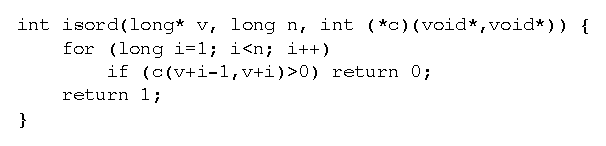
\includegraphics[width=0.66\textwidth]{figures/osr-isord/osr-isord.eps}
\caption{\protect\label{fig:osr-isord} Example for OSR instrumentation in LLVM.
}
\end{center}
\end{figure}
\fi

\ifdefined\noauthorea
\begin{figure}[!ht]
\begin{center}
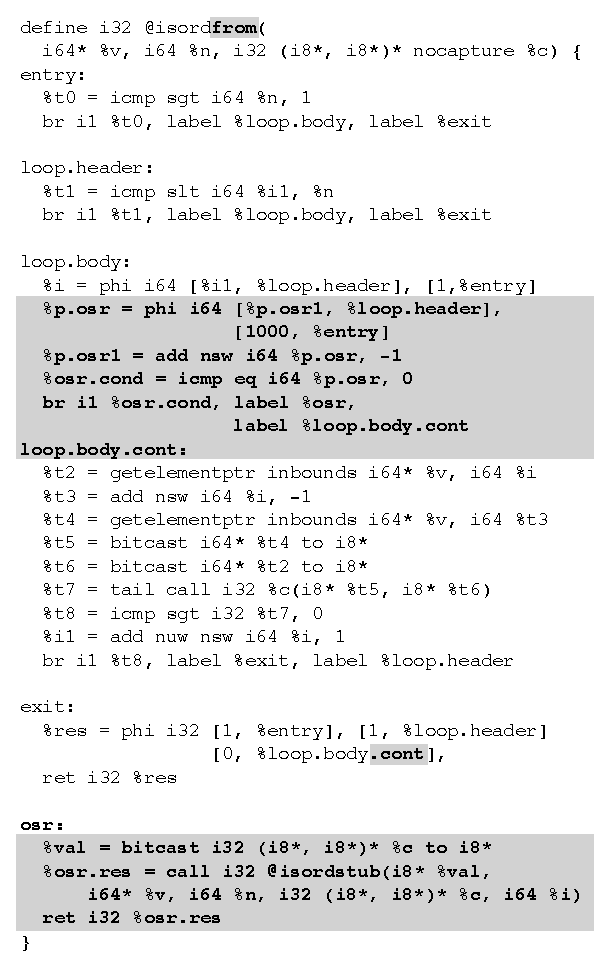
\includegraphics[width=0.66\textwidth]{figures/osr-isordfrom/osr-isordfrom.eps}
\caption{\protect\label{fig:osr-isordfrom} LLVM IR version of base function {\tt isord} (\myfigure\ref{fig:osr-isord}) instrumented for open OSR. Additions resulting from the instrumentation are in grey. The OSR is fired at the beginning of the loop body after 1000 iterations, i.e., when the counter reaches 0.

}
\end{center}
\end{figure}
\fi

\paragraph*{IR Instrumentation.}
To defer the compilation of the continuation function until the comparator is known at run time, we used \osrkit\ to instrument {\tt isord} with an open OSR point at the beginning of the loop body, as shown in \myfigure\ref{fig:osr-isordfrom}. Portions added to the original code by OSR instrumentation are highlighted in grey.

New instructions are placed at the beginning of the loop body to increment a hotness counter {\tt p.osr} and jump to an OSR-firing block if the counter reaches the threshold (1000 iterations in this example). The OSR block contains a tail call to the target generation stub, which receives as parameters the four live variables at the OSR point ({\tt v}, {\tt n}, {\tt c}, {\tt i}). \osrkit\ allows the stub to receive the run-time value {\tt val} of an IR object that can be used to produce the continuation function -- in our example, the pointer to the comparator function to be inlined. The stub (shown in \myfigure\ref{fig:osr-isordstub}) calls a code generator that:
\begin{enumerate}[parsep=0pt,itemsep=3pt]
 \item builds an optimized version of {\tt isord} by inlining the comparator, and
 \item uses it to create the continuation function {\tt isordto} shown in \myfigure\ref{fig:osr-isordto}.
\end{enumerate}

\noindent The stub passes to the code generator four parameters:
\begin{enumerate}[parsep=0pt,itemsep=3pt]
 \item a pointer to the {\tt isord} IR code;
 \item a pointer to the basic block in {\tt isord} from which the OSR is fired;
 \item a pointer to a user-defined object to support code generation in MCJIT;
 \item the stub's {\tt val} parameter.
\end{enumerate}

\noindent The first three parameters are provided by the front-end and hard-wired by \osrkit. In particular, the third parameter is a handle to the environment for code generation (e.g., in our dynamic inliner the object contains pointers to the MCJIT engine and to a map between addresses of compiled functions and their IR counterparts). The stub terminates with a tail call to {\tt isordto}.

\ifdefined\noauthorea
\begin{figure}[ht]
\begin{center}
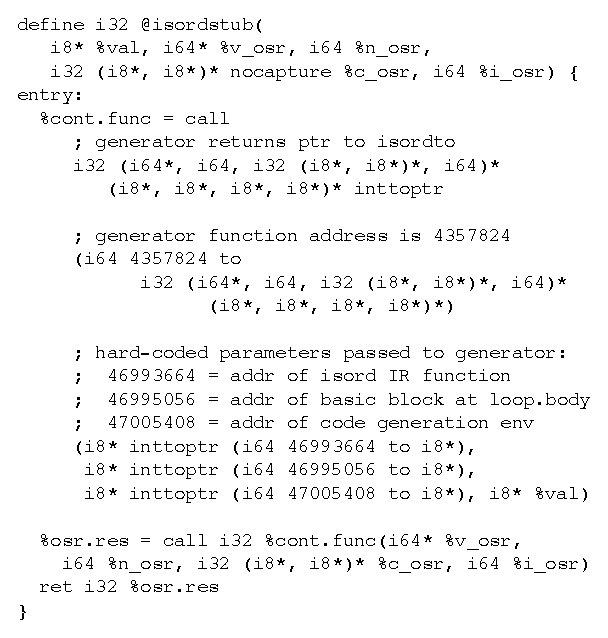
\includegraphics[width=0.66\textwidth]{figures/osr-isordstub/osr-isordstub.eps}
\caption{\protect\label{fig:osr-isordstub} IR stub that generates the continuation function when an open OSR is fired by {\tt isordfrom} (\myfigure\ref{fig:osr-isordfrom}).
}
\end{center}
\end{figure}
\fi

\noindent To generate the continuation function (shown in \myfigure\ref{fig:osr-isordto}) from the optimized version created by the inliner, \osrkit\ replaces the function entry point, removes dead code, replaces live variables with the function parameters, and fixes $\phi$-nodes accordingly. As the OSR transition does not require any modification to the program state, the new entry point does not contain any form of compensation code. Preserving the SSA form while constructing the continuation function is a challenging task, as it might require inserting new $\phi$-nodes in the control-flow graph in addition to simply updating some of the existing ones as in this example. When generating a continuation function, we rely on the {\tt SSAUpdater} component of LLVM to account for the available values -- transferred as parameters or reconstructed in the OSR entrypoint -- of all the variables that are live at the OSR landing pad.

%Additions resulting from the IR instrumentation are in grey, while removals are struck-through.

\ifdefined\noauthorea
\begin{figure}[ht]
\begin{center}
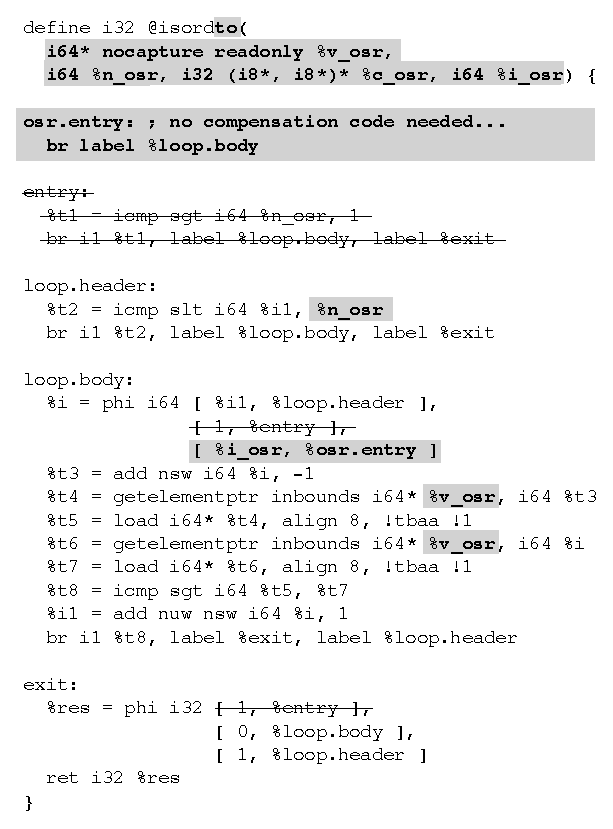
\includegraphics[width=0.66\columnwidth]{figures/osr-isordto/osr-isordto.eps}
\caption{\protect\label{fig:osr-isordto} Faster variant of {\tt isord} (\myfigure\ref{fig:osr-isord}) in LLVM IR with comparator inlining, instrumented as OSR continuation function. Instrumentation additions are in grey. The original function entry block is unreachable after instrumentation and is eliminated (struck-through code fragments).
}
\end{center}
\end{figure}
\fi


\subsection{Discussion}
Instrumenting functions for OSR at a higher level than machine code yields several benefits: 
\begin{enumerate}[parsep=0pt]
\item {\em Platform independence}: the OSR instrumentation code is lowered to native code by the compiler back-end, which handles the details of the target ABI. 
\item {\em Global optimizations}: lowering OSR instrumentation code along with application code can generate faster code than local binary instrumentation. For instance, dead code elimination can suppress from \fosrto\ portions of code that would no longer be needed when jumping to the landing pad \textsf{L'}, producing smaller code and enabling better register allocation and instruction scheduling.
\item {\em Debugging and Profiling}: preserving ABI conventions in the native code versions of \fosrfrom, \fstub, and \fosrto\ helps debuggers and profilers to more precisely locate the current execution context and collect more informative data.
%avoiding low-lever tampering with stack frames can more easily preserve ABI calling conventions
\item {\em Abstraction}: being entirely encoded using high-level language constructs (assignments, conditionals, function calls), the approach is amenable to a clean instrumentation API that abstracts the OSR implementation details, allowing a front-end to focus on where to insert OSR points independently of the final target architecture.
%by analyzing code at an intermediate representation level.
\end{enumerate}

\noindent A natural question is whether encoding OSR at a higher level of abstraction can result in poorer performance than binary code approaches. Our solution relies on the backend's compilation pipeline to generate the most efficient native code for \fosrfrom\ and \fosrto. In the next section, we present an implementation of our framework in the LLVM compiler infrastructure, showing examples of OSR machine code generated for an x86-64 target. We then provide performance numbers in Section\missing, where OSR performance is measured on classic benchmarks.

\mynote{Compensation code, OSR at arbitrary points, effort to investigate its feasibility}

